\subsection{Huấn luyện mô hình HMM}
\subsubsection{Tập dữ liệu huấn luyện}
Tập dữ liệu huấn luyện sau khi trích suất đặc trưng:

\begin{itemize}
    \item Tổng số chiều (D): 39
    \item Global Mean (TB của các chiều): -0.0000
    \item Global Std Dev (TB của các chiều): 1.0000
\end{itemize}

\begin{figure}[ht]
    \centering
    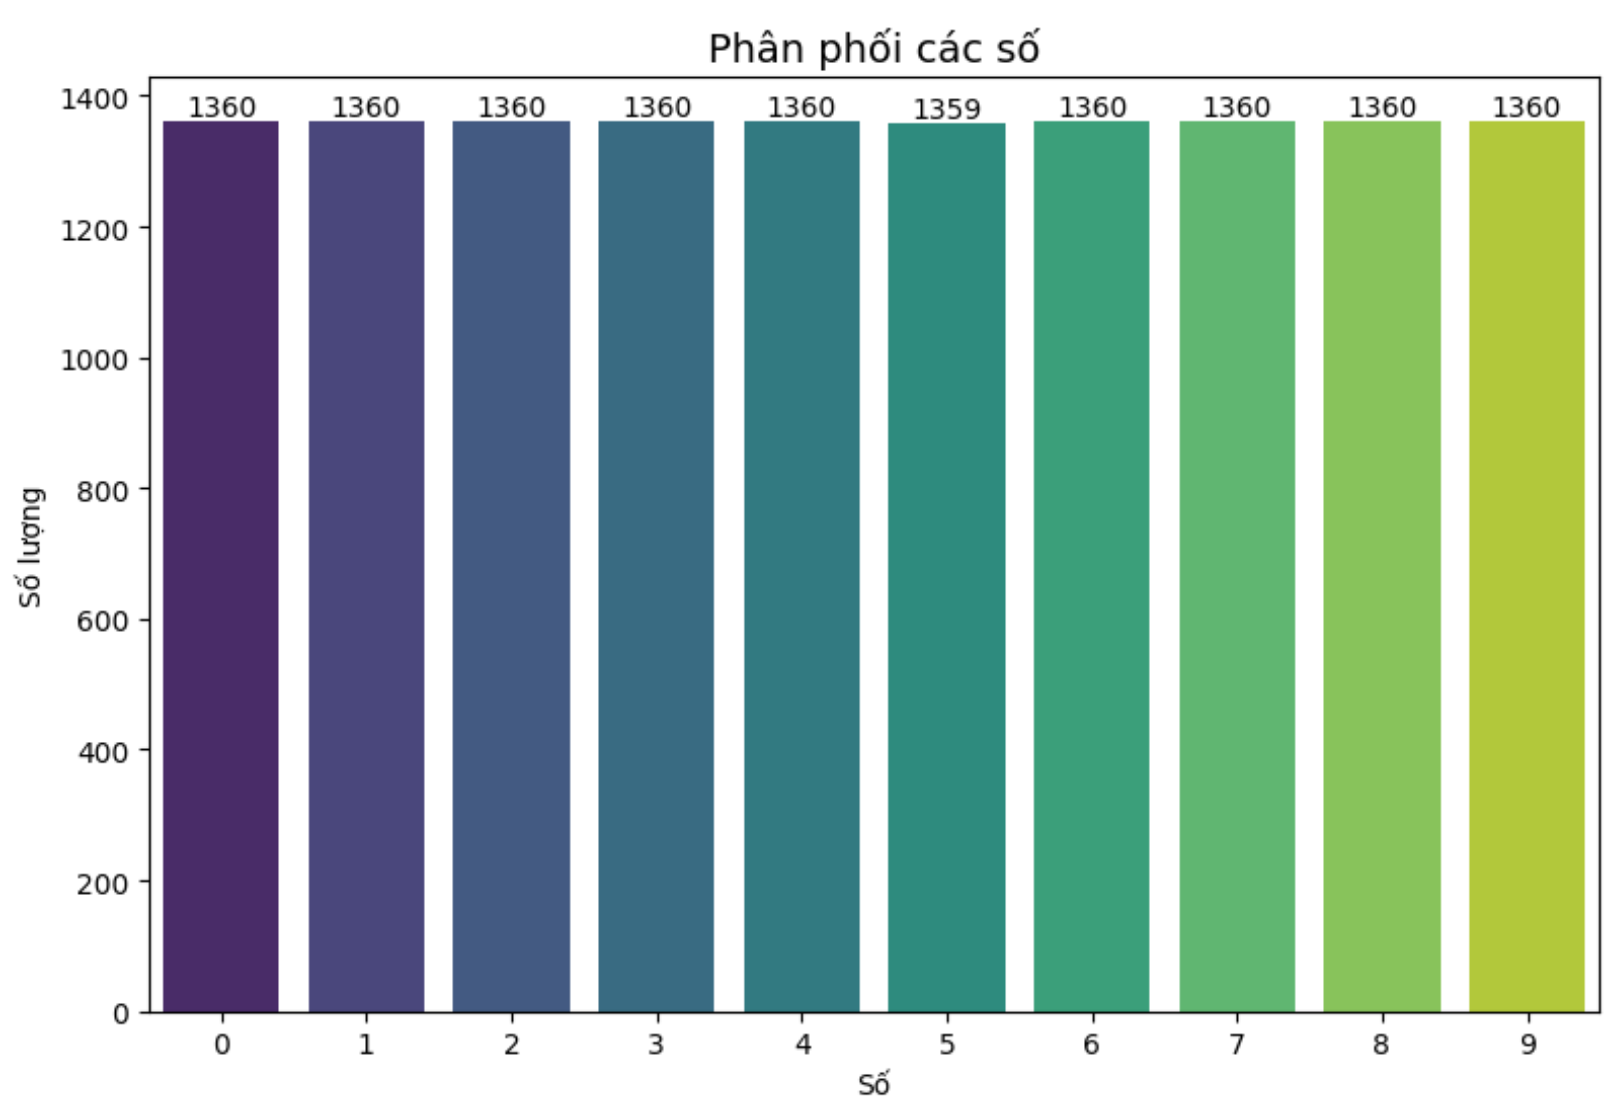
\includegraphics[width=1.0\textwidth]{graphics/X_train1.png}
    \caption{Phân phối của tập dữ liệu huấn luyện sau khi trích suất đặc trưng MFCC}
    \label{fig:train_data_quantity}
\end{figure}

\begin{figure}[ht]
    \centering
    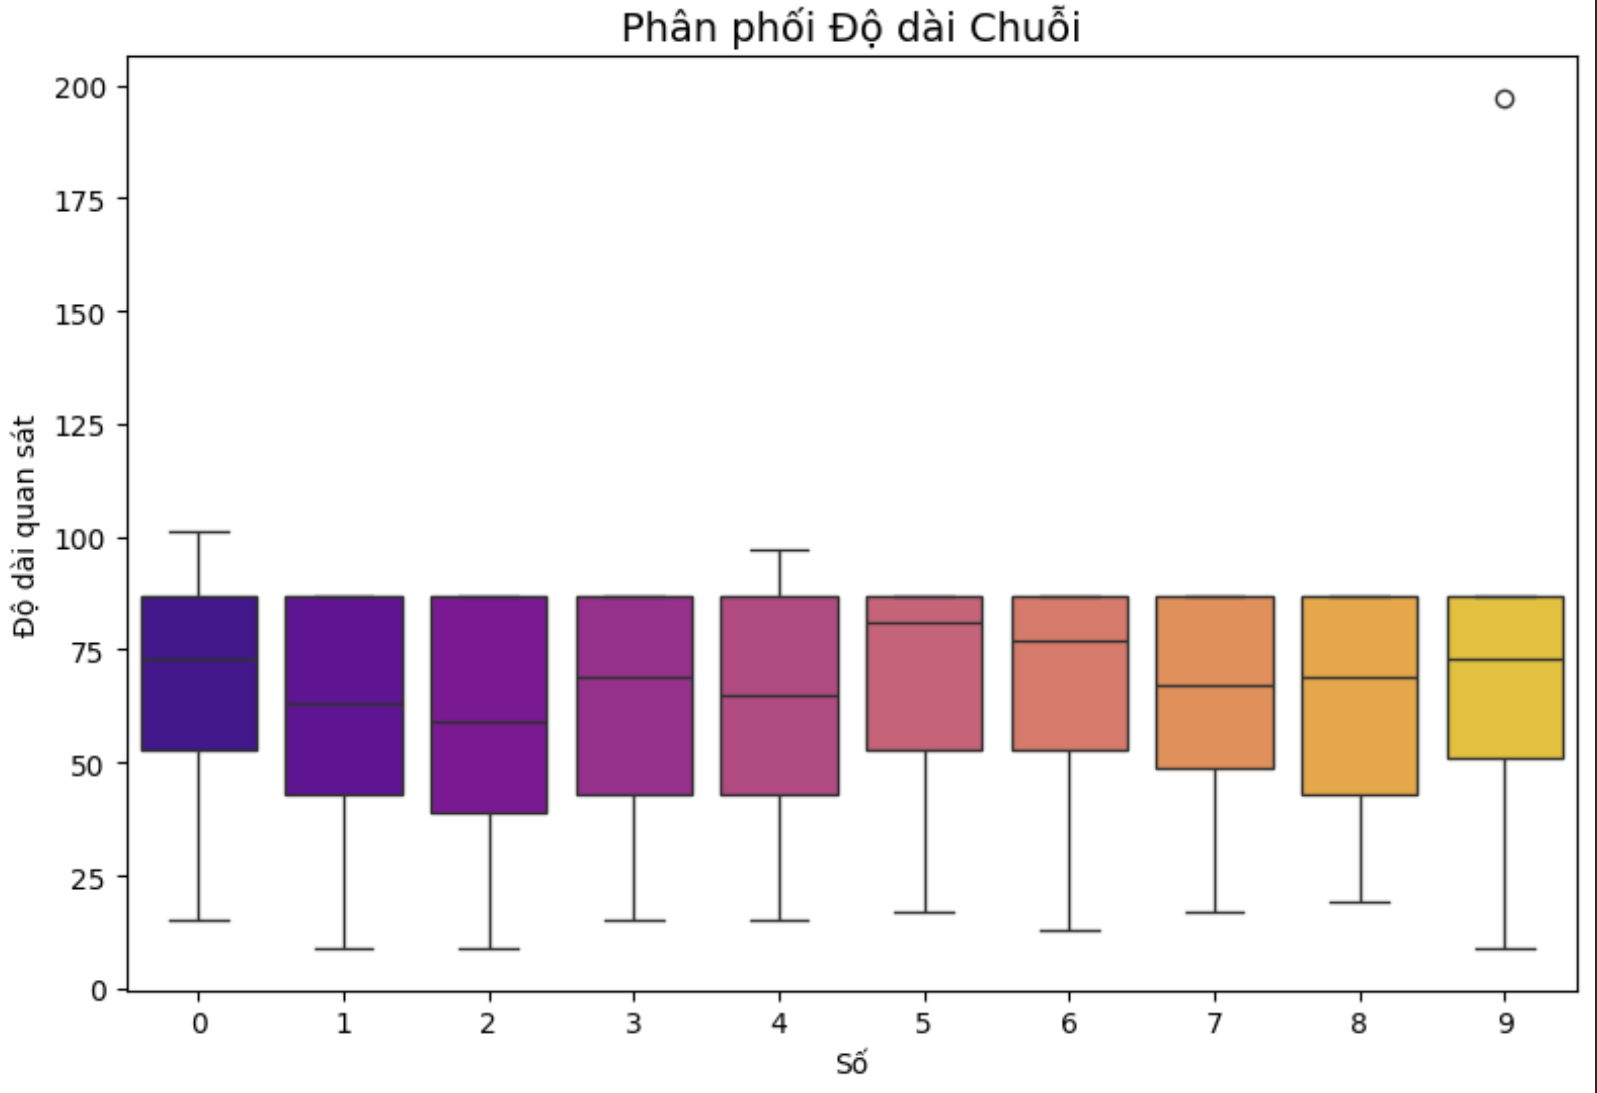
\includegraphics[width=1.0\textwidth]{graphics/X_train2.png}
    \caption{Độ dài của tập dữ liệu huấn luyện sau khi trích suất đặc trưng MFCC}
    \label{fig:train_data_length}
\end{figure}

\break

\subsubsection{Phương pháp xây dựng mô hình}
Tập dữ liệu huấn luyện trên có giá trị liên tục xấp xỉ phân phối Gaussian do đó phương pháp để xây dựng mô hình giải quyết là:

\begin{itemize}
    \item Tách tập train thành 10 tập tương ứng với 10 chữ số từ 0 đến 9.
    \item Sử dụng mô hình continueHMM với hàm phát xạ là hàm Gaussian.
    \item Sử dụng thuật toán Baum-Welch huấn luyện 10 mô hình tương ứng với các tập.
    \item Khi kiểm tra, sử dụng hàm Forward để tính xác suất quan sát thuộc về từng mô hình. Lấy mô hình có xác suất cao nhất làm nhãn dự đoán.
\end{itemize}

\subsubsection{Hiện thực hàm huấn luyện mô hình}

\subsubsection*{Khởi tạo tham số đầu vào:}

\textbf{Tham số đầu vào} cho hàm huấn luyện bao gồm:
\begin{itemize}
    \item Số trạng thái ẩn N.
    \item Số vòng lặp tối đa N\_loop
    \item Ngưỡng hội tụ epsilon
\end{itemize}

\textbf{Khởi tạo tham số} của mô hình HMM bao gồm:
\begin{itemize}
    \item Khởi tạo \(\pi\) theo phân phối đều.
    
\begin{tcolorbox}
\begin{lstlisting}[language=Python]
    pi = np.full(num_states, 1.0/num_states)
\end{lstlisting}
\end{tcolorbox}

    \item Ma trận chuyển trạng thái A được khởi tạo theo mô hình left-right \ref{[1]} với bậc chuyển trạng thái là 2. Do mô hình tập trung vào giải quyết nhận dạng chữ số, các trạng thái ẩn sẽ được sắp xếp theo trình tự thời gian từ trái sang phải. Mỗi trạng thái chỉ có thể chuyển sang chính nó hoặc hai trạng thái tiếp theo.

\begin{tcolorbox}
\begin{lstlisting}[language=Python]
A = np.zeros((num_states, num_states))
    for i in range(num_states):
        stay = 0.6
        move = 0.4
        if i == num_states - 1:
            A[i, i] = 1.0
        else:
            A[i, i] = stay
            A[i, i+1] = move
A /= A.sum(axis=1, keepdims=True)
\end{lstlisting}
\end{tcolorbox}

    \item Tham số mean được khởi tạo ngẫu hiện theo phân phối chuẩn với mean = 0 và std = 1. Do tập dữ liệu huấn luyện đã được chuẩn hóa.
    
\begin{tcolorbox}
\begin{lstlisting}[language=Python]
    means = np.random.randn(num_states, D)
\end{lstlisting}
\end{tcolorbox}

    \item Tham số covariance được khởi tạo là ma trận hiệp phương sai chéo với giá trị trên đường chéo là phương sai toàn cục của tập dữ liệu huấn luyện cộng một hằng số nhỏ 1e-3 để tránh trường hợp ma trận không khả nghịch.
\begin{tcolorbox}
\begin{lstlisting}[language=Python]
    global_var = np.var(X, axis=0) + 1e-3
    covariances = np.zeros((num_states, D, D))
    for s in range(num_states):
        covariances[s] = np.diag(global_var)
\end{lstlisting}
\end{tcolorbox}
\end{itemize}

\subsubsection*{Chạy hàm fit đã để huấn luyện mô hình}

Với hàm init\_params là hàm khởi tạo ra các tham số ở trên.

\begin{tcolorbox}
\begin{lstlisting}[language=Python]
    models = []
    for cls_id, cls_name in enumerate(class_names):
        seq_list = [X_train[i] for i, y in enumerate(y_train) if y == cls_id]
        A, pi, means, covs = _init_params(num_states, seq_list)
        model = continueHMM(A=A, means=means, covariances=covs, pi=pi).fit(seq_list, n_loop=n_loop, bound_learning=tol)
        models.append(model)
\end{lstlisting}
\end{tcolorbox}

\subsubsection{Hiện thực hàm kiểm tra}
Sau khi huấn luyện xong 10 mô hình tương ứng với 10 chữ số, ta sử dụng hàm Forward để tính xác suất quan sát thuộc về từng mô hình. Lấy mô hình có xác suất cao nhất làm nhãn dự đoán.

\begin{tcolorbox}
\begin{lstlisting}[language=Python]
    y_pred = []
    for seq in X_test:
        scores = [m.forward(seq)[0] for m in models]
        y_pred.append(int(np.argmax(scores)))
\end{lstlisting}
\end{tcolorbox}

\subsection{Đánh giá mô hình}

Sau khi huấn luyện mô hình HMM và kiểm tra trên tập dữ liệu test, ta thu được kết quả như sau:

% --- Tổng kết ---
\subsubsection*{Tổng Kết Kết Quả}

\begin{itemize}
    \item Accuracy (Global):  0.9271
    \item Precision Macro:    0.9285
    \item Precision Weighted: 0.9285
    \item Recall Macro:       0.9271
    \item Recall Weighted:    0.9271
    \item F1 Macro:           0.9271
    \item F1 Weighted:        0.9271
\end{itemize}

\break

% --- Ma trận nhầm lẫn ---
\subsubsection*{Ma Trận Nhầm Lẫn}
\begin{figure}[ht]
    \centering
    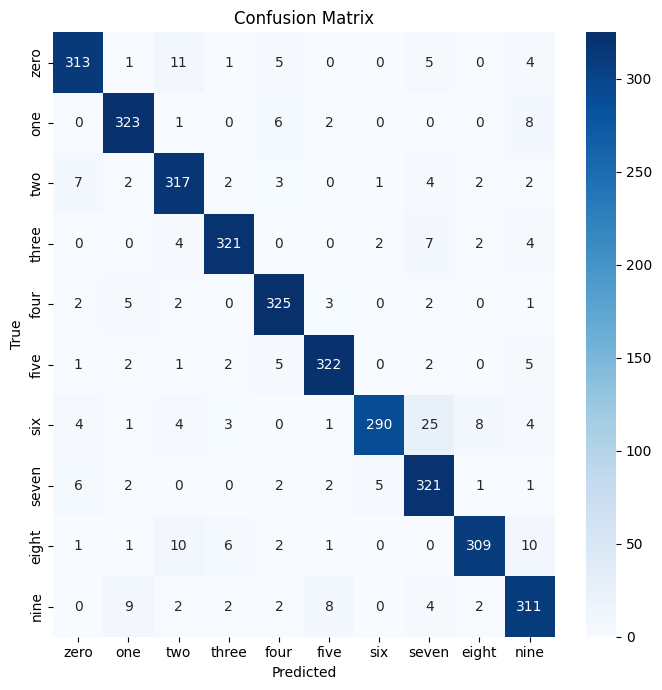
\includegraphics[width=0.8\textwidth]{graphics/confuse.png}
    \caption{Ma trận nhầm lẫn của mô hình HMM trên tập dữ liệu kiểm tra}
    \label{fig:confusion-matrix}
\end{figure}

\break

% --- Báo cáo đánh giá chi tiết (ĐÃ GỘP) ---
\subsubsection*{Báo Cáo Đánh Giá Chi Tiết}

% [htbp] là tùy chọn vị trí tốt (here, top, bottom, page)
\begin{table}[ht] 
\centering
\caption{Báo cáo đánh giá chi tiết}
\label{tab:detailed-report}
\begin{tabular}{l r r r r r r}
\toprule
\textbf{Lớp} & \textbf{Precision} & \textbf{Recall} & \textbf{F1-Score} & \textbf{Accuracy} & \textbf{Correct} & \textbf{Support} \\
\midrule
zero         & 0.94 & 0.92 & 0.93 & 92.06\% & 313 & 340 \\
one          & 0.93 & 0.95 & 0.94 & 95.00\% & 323 & 340 \\
two          & 0.90 & 0.93 & 0.92 & 93.24\% & 317 & 340 \\
three        & 0.95 & 0.94 & 0.95 & 94.41\% & 321 & 340 \\
four         & 0.93 & 0.96 & 0.94 & 95.59\% & 325 & 340 \\
five         & 0.95 & 0.95 & 0.95 & 94.71\% & 322 & 340 \\
six          & 0.97 & 0.85 & 0.91 & 85.29\% & 290 & 340 \\
seven        & 0.87 & 0.94 & 0.90 & 94.41\% & 321 & 340 \\
eight        & 0.95 & 0.91 & 0.93 & 90.88\% & 309 & 340 \\
nine         & 0.89 & 0.91 & 0.90 & 91.47\% & 311 & 340 \\
\midrule
% Dòng accuracy tổng thể
\textbf{accuracy}     &      &      & \textbf{0.93} & & & \textbf{3400} \\
\textbf{macro avg}    & 0.93 & 0.93 & 0.93 & & & 3400 \\
\textbf{weighted avg} & 0.93 & 0.93 & 0.93 & & & 3400 \\
\bottomrule
\end{tabular}
\end{table}

\subsection{Kết luận}
\subsubsection{Ưu điểm}
\begin{itemize}
    \item Mô hình HMM với hàm phát xạ Gaussian phù hợp với bài toán nhận dạng chữ số sử dụng dữ liệu liên tục.
    \item Kết quả đạt được khá tốt với độ chính xác trên 92\%.
    \item Hiện thực mô hình bằng numpy giúp việc triển khai nhanh chóng và dễ dàng điều chỉnh các tham số của mô hình.
    \item Mô hình có thể mở rộng để nhận dạng các loại dữ liệu khác nhau bằng cách thay đổi hàm phát xạ.
    \item Mô hình có thể được cải thiện thêm bằng cách tăng số trạng thái ẩn hoặc sử dụng các hàm phát xạ phức tạp hơn như Gaussian hỗn hợp.
    \item Mô hình có thể được áp dụng trong các ứng dụng thực tế như nhận dạng giọng nói, nhận dạng chữ viết tay, và các hệ thống nhận dạng mẫu khác.
\end{itemize}
\subsubsection{Nhượt điểm}
\begin{itemize}
    \item Mô hình HMM giả định rằng các quan sát là độc lập và tuân theo phân phối Gaussian, điều này có thể không phản ánh đúng bản chất của dữ liệu thực tế.
    \item Việc lựa chọn số trạng thái ẩn và các tham số khác của mô hình có thể ảnh hưởng lớn đến hiệu suất của mô hình, và việc tìm kiếm các tham số tối ưu có thể tốn thời gian và công sức.
    \item Mô hình HMM có thể gặp khó khăn trong việc xử lý các chuỗi quan sát dài hoặc phức tạp, dẫn đến hiệu suất kém hơn so với các mô hình học sâu hiện đại.
    \item Việc huấn luyện mô hình HMM có thể bị ảnh hưởng bởi các vấn đề như overfitting hoặc underfitting, đặc biệt khi tập dữ liệu huấn luyện không đủ lớn hoặc đa dạng.
    \item Mô hình HMM có thể không hiệu quả trong việc xử lý các dữ liệu có nhiều biến động hoặc nhiễu, dẫn đến kết quả nhận dạng không chính xác.
\end{itemize}